%++++++++++++++++++++++++++++++++++++++++
\documentclass[letterpaper,12pt]{article}
\usepackage[ngerman,english]{babel}
\usepackage{siunitx} 
\usepackage{tabularx} % extra features for tabular environment
\usepackage{amsmath}  % improve math presentation
\usepackage{graphicx} % takes care of graphic including machinery
\usepackage[margin=1in,letterpaper]{geometry} % decreases margins
\usepackage{cite} % takes care of citations
\usepackage[final]{hyperref} % adds hyper links inside the generated pdf file
\usepackage{xcolor}
\hypersetup{
	colorlinks,
	linkcolor={red!50!black},
	citecolor={blue!50!black},
	urlcolor={blue!80!black}
}
%++++++++++++++++++++++++++++++++++++++++


\begin{document}
	
	\selectlanguage{ngerman}
	\title{Hochfrequenzchirurgie}
	\author{Heinrich Merk}
	\date{\today}
	\maketitle
	
	\selectlanguage{english}
	\begin{abstract}
		In dieser Ausarbeitung geht es um die Hochfrequenzchirurgie und derer grundlegenden physikalischen Prozesse. Es werden die verschiedenen Auswirkungen auf das Gewebe, die Apparatur sowie das grundlegende Verständis zur dahinter liegenden Technik beleuchtet. Zum Schluss werden neu erworbene Techniken aufgegriffen und Aussichtsmöglichkeiten vorgestellt.
		
	\end{abstract}
	
	\selectlanguage{ngerman}
	\section{Einleitung}
	
		Unter der Hochfrequenzchirurgie versteht man den assistierenden Einsatz von elektrischer Energie in der Chirurgie zur thermisch induzierten Veränderung oder Zerstörung von Gewebezellen mit dem Ziel der Hämostase (Blutstillung), Gewebedurchtrennung oder -versiegelung \cite{kramme2016medizintechnik}. Durch die kompakte Größe der Geräte, die einfache Handhabung und der Preiswertigkeit hat sich die HF-Chirurgie zu einem unentbehrlichen Handwerkszeug im operativen Alltagsbereich entwickelt und ist kaum noch wegzudenken.
	
	\section{Stand der Technik}
	
		Die HF-Chirurgie lässt sich grundsätzlich auf drei wichtige Bauteile, dem \emph{Hochfrequenzgenerator}, dem \emph{Handstück mit Applikator} und der \emph{Erdung} beschränken. Hierbei sorgt der HF-Generator für den benötigten Wechselstrom in einer wohl definierten Frequenz. Diese sind in der Lage eine Frequenz von $f>\SI{300}{\kilo\hertz}$ zu betreiben. Applikatoren als Handwerkszeug und Stromspitze können je nach Anwendung in verschiedenen Bauformen auftreten. Hier kann ein isoliertes Handstück diverse Applikatorspitzen für den jeweiligen Einsatz aufnehmen. Die Erdung erfolgt mithilfe einer großflächigen Elektrode, einer Negativspitze (Pinzette) oder aber der Patientenstuhl ist als Erdung direkt konfiguriert. 
		
	
	\newpage
	\section{Grundlagen}
	
		\subsection{Thermische Prozesse im Gewebe}
		
		Das Gewebe besteht grundsätzlich aus Proteinbausteinen, welche durch Temperaturerhöhung eine veränderte Form erfahren. Dabei sind folgende Stufen für die Hochfrequenzchirurgie von Relevanz:
		\begin{itemize}
			\item $37^\circ-45^\circ$ $\Rightarrow$ Erwärmung des Gewebes
			\item $45^\circ-70^\circ$ $\Rightarrow$ Proteindenaturierung (3D-Struktur der Proteine geht verloren, d.h. auch ihre Funktion)
			\item $70^\circ-100^\circ$ $\Rightarrow$ Koagulation (Verklumpen von Proteinen)
			\item $100^\circ-300^\circ$ $\Rightarrow$ Karbonisation (Gewebe trocknet aus)
			\item über $300^\circ$ $\Rightarrow$ Verdampfen und Abtragung des Gewebes
		\end{itemize}
		Bereits bei der Proteindenaturisierung sterben die Zellen ab und sind nicht mehr in der Lage sich selbstständig zu regenerieren. Die anschließende Koagulation findet Einsatz in der Blutstillung. Durch das verklumpen der Proteine wird eine Blutgerinnung verhindert...
	
		\subsection{Elektrische Wechselwirkung mit dem Gewebe}
	
			Fließt ein elektrischer Strom durch biologisches Gewebe, treten je nach Stromart, Stromstärke und Frequenz drei unterschiedliche Effekte auf:
			\paragraph{Gleichstrom ($f=\SI{0}{\hertz}$)}
			Gleichstrom hat für das Gewebe eine elektrolytische Wirkung. Es folgt eine Ionenverschiebung und elektrochemische Prozesse treten in Kraft. 
			\paragraph{Wechselstrom ($f=\SI{20}{\hertz}-\SI{20}{\kilo\hertz}$)}
			Bei diesen Frequenzen treten faradische Effekte auf. Diese sorgen für eine Störung der Nerven- und Muskelreizung. Gefährlich sind solche Frequenzen insbesondere für das Herz, da diese es kontrahieren lassen und Herzrythmusstörungen zur Folge haben.
			\paragraph{Wechselstrom ($f=\SI{300}{\kilo\hertz}-\SI{4}{\mega\hertz}$)}
			Derartige Frequenzen lassen thermische Effekte zu. Die elektrische Energie kann effektiv übertragen werden, da hohe Frequenzen für eine hohe Leitfähigkeit im Gewebe sorgen, das vor allem einen kapazitiven Widerstand hat. Die obere Grenze des Frequenzbereichs ist durch die kapazitiven Ableitströme der Elektroden und Kabel bestimmt. Mit steigender Frequenz wird auch verstärkt und unerwünscht Energie abgestrahlt und die Beherrschung der Wirkung wird problematischer. Die Gefahr, den Patienten durch Verbrennungen an anderer Stelle zu verletzen, würde steigen.\\\\	
			Die Erwärmung des Gewebes ist abhängig von der Stromdichte, welche wie folgt definiert ist:
			\begin{equation} \label{eq:stromdichte}
				S=\frac{I}{A}
			\end{equation}
			Die Einwirkfläche $A$ wird von der Geometrie der Applikatoren, welche letztendlich mit der Haut in Kontakt kommen, bestimmt. Eine spitze Form sorgt für eine kleine Fläche und folglich einer hohen Stromdichte $S$. Anwendungsgebiet ist das Schneiden von Gewebe. Eine beispielsweise kugelförmige Geometrie sorgt hingegen für eine geringere Stromdichte. Dadurch kann eine Koagulation des Gewebes erfolgen.\\Der Strom $I$ hängt ab vom spezifischen Widerstand des Gewebes und der verwendeten Effektivspannung
			\begin{equation} \label{eq:effektivspannung}
			U_{effektiv}=R_{Gewebe} \cdot I.
			\end{equation}
			Auch die Einwirkzeit hat einen Einfluss auf die Erwärmung des Gewebes. Je länger der Wärmefluss ins Gewebe andauert, desto höher ist der Temperaturanstieg. Mit steigender Temperatur ändert sich wiederum der Gewebezustand.
		
		\subsection{Schneiden und Koagulation}
		
			Die zwei grundlegenden Gewebeeffekte der HF-Chirurgie, das Schneiden und Koagulieren, beinhalten das Erhitzen des leitfähigen Gewebes durch einen hochfrequenten elektrischen Strom, der im Falle des Schneidens zu einer Verdampfung und Ionisierung des Wassergehalts in Geweben führt, was mit einer Sinuswelle erreicht wird, die zu extremen Spitzen des Temperaturanstiegs führt. Je nach Anwendung können unterschiedliche Arten von Schnitten mithilfe modulierter Ströme hervorgerufen werden, die zu einer gewissen Abkühlung des Gewebes führen. Dabei unterscheidet man, je nach durch der Modulation hervorgerufener Glätte, zwischen \emph{pure cut}, \emph{blend cut} und \emph{super blend cut}.
			
			Die Koagulation des Gewebes geht aus der thermischen Denaturierung ohne Gewebeverdampfung hervor. Dies wird durch eine Reihe diskontinuierlicher Wellenpakete erreicht, bei denen Ruhephasen die sinusförmigen Wellenzyklen unterbrechen und die Gewebebildung ein wenig abkühlen lassen. 
			
			Abbildung \ref{fig:schneidenStrom} zeigt die verschiedenen Modulationen und deren Auswirkung auf das Gewebe und Abbildung \ref{fig:koagulationStrom} verdeutlicht den Sachverhalt anhand einer Probe.
\begin{figure}[ht]
	\centering
	\begin{minipage}[t]{0.45\linewidth}
		\centering
		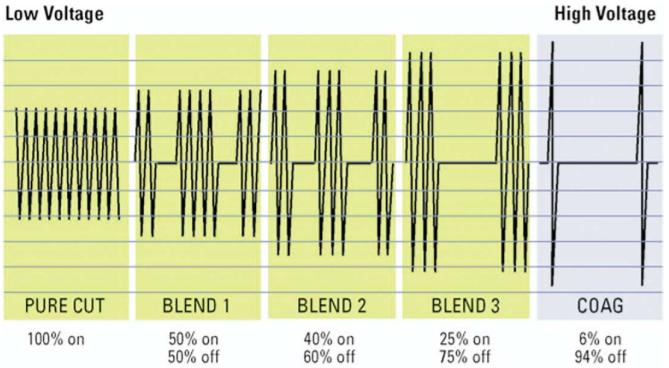
\includegraphics[width=\linewidth]{images/_stromModi.png}
		\caption{Je nach erforderlicher Gröbe des Schnittes wird der Strom gepulst moduliert. Beim Koagulieren (rechts) wird eine hohe Effektivspannung benutzt und lange Pausen in der Modulation angewendet \cite{stromModi}.}
		\label{fig:schneidenStrom}
	\end{minipage}
	\hfill
	\begin{minipage}[t]{0.45\linewidth}
		\centering
		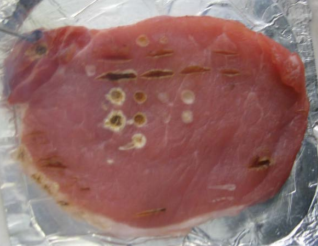
\includegraphics[width=5cm]{images/fleisch.png}
		\caption{Im oberen Bereich sind die einzelnen Stufen der Schnittgröbe zu sehen. Beim Koagulieren wiederum entstehen großflächige Denaturierungen und das Gewebe verfärbt sich allmählich.}
		\label{fig:koagulationStrom}
	\end{minipage}
\end{figure}
		
	\section{Anwendung}
	
		Die verschiedenartigen Anwendungsformen können prinzipiell in \emph{bipolare und monopolare Verfahren} eingeteilt werden. Die monopolare Anwendungstechnik kommt dabei am häufigsten zum Einsatz \cite{kramme2016medizintechnik}.
		
		\subsection{Bipolare Technik}
		
			Für die Erzeugung eines elektrischen Stroms benötigt man grundsätzlich zwei Elektroden mit je einem +Pol und -Pol. Bei der bipolaren Technik besitzt der Applikator zwei Spitzen, ähnlich einer Pinzette, zwischen denen die Spannung anliegt. Das zu bearbeitende Gewebe wird zwischen den Pinzettenspitzen genommen und stellt so einen Stromfluss durch das Gewebe her. Abbildung \ref{fig:bipolareTechnik2} veranschaulicht das Prinzip.
			\begin{figure}[ht] 
				\centering
				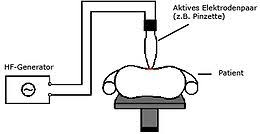
\includegraphics[width=0.35\columnwidth]{images/_bipolareTechnik.png}
				\caption{		 
					Bipolarer Stromkreis: Der Stromfluss bleibt auf das zwischen den beiden Pinzettenspitzen gefasste Gewebe begrenzt \cite{wiki:HF}.}
				\label{fig:bipolareTechnik2}
			\end{figure}\\
			Bipolare Instrumente gewinnen immer mehr an Bedeutung, da der Stromweg zwischen den Elektrodenspitzen kalkulierbar ist und nicht weite Strecken durch den Körper des Patienten durchläuft. Damit reduziert sich die Beeinflussung von beispielsweise Herzschrittmachern oder sonstigen Geräten, die während der Operation an dem Patienten angeschlossen sind.
		
		\subsection{Monopolare Technik}
		
			Bei der monopolaren Technik fließt der Strom zwischen Applikatorelektrode und einer großflächigen Gegenelektrode, wobei die Stromdichte an der Applikatorelektrode sehr hoch ist, sodass thermische Effekte auftreten.
			Die Stromdichte nimmt hin zur Aktiven Elektrode quadratisch zu, das bedeutet außerhalb des Wechselwirkungvolumens fächern sich die E-Feldlinien derart auf, dass die Stromdichte für nicht relevante Körperstellen unkritisch ist. Dieser Sachverhalt wird in Abbildung \ref{fig:monopolareTechnik2} deutlich. Wichtig ist hierbei die gewissenhafte Aufbringung der Gegenelektrode. Es darf des weiteren keine Berührung durch dritte Personen während der Behandlung auftreten.
			\begin{figure}[h!] 
				\centering
				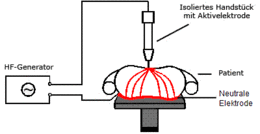
\includegraphics[width=0.35\columnwidth]{images/_monopolareTechnik.png}
				\caption{		 
					Monopolarer Stromkreis mit am Oberschenkel des Patienten angelegter, großflächiger Neutralelektrode \cite{wiki:HF}.}
				\label{fig:monopolareTechnik2}
			\end{figure}\\
			Zu erwähnen sei auch noch die monoterminale Technik, bei der sich nach Abbildung \ref{fig:monoterminaleTechnik} der Stromkreis über die Kapazität des Patientenkörpers zu dessen geerdeter Unterlage schließt. Dies ermöglicht ein Operieren ohne vorheriges Aufbringen der Gegenelektrode. Jedoch ist diese Technik nur für den Bereich kleiner Ströme geeignet und kommt daher für kleinere Eingriffe wie in der Zahnheilkunde oder Dermatologie in Frage. 
			\begin{figure}[h!] 
				\centering
				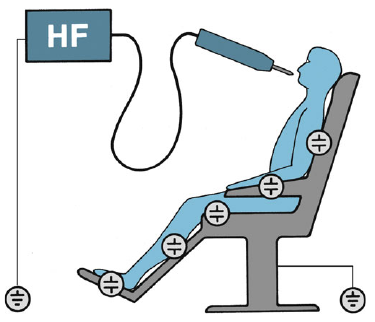
\includegraphics[width=0.35\columnwidth]{images/monoterminaleTechnik.png}
				\caption{		 
					Monopolarer Stromkreis mit am Oberschenkel des Patienten angelegter, großflächiger Neutralelektrode \cite{kramme2016medizintechnik}.}
				\label{fig:monoterminaleTechnik}
			\end{figure}\\

			
		\subsection{Weiterführende Anwendungen}
			
			Eine weitere Anwendung in der HF-Chirurgie ist das \emph{Argonassistierte Schneiden}. Hierbei wird während der Anwendung ein Schutzgas (Argon) benutzt um den Luftsauerstoff aus dem Wechselwirkungsvolumen zu verdrängen und eine Schutzatmosphäre zu bilden. Aus dem Applikatorschaft ragt dann eine aktive Schneideelektrode, die beim Schneidevorgang von Argongas koaxial umströmt wird. Dies hat eine Reduzierung der Karbonisierung und somit einen besseren Heilungsverlauf zur Folge. Außerdem verbessert sich die Sicht des Operateurs zum Wechselwirkungsvolumen aufgrund minimierter Rauchbildung. Anwendungsgebiete sind die Dermatologie und allgemeine Weichteilchirurgie.
					
			Die HF-Chirurgie ist für Hartgewebe wie Knochen oder Knorpel nicht geeignet, da die Leitfähigkeit aufgrund fehlendem Gewebewasser zu gering ist. Nach Gleichung \ref{eq:effektivspannung} wäre $R_{Gewebe}$ zu groß, sodass sich kein vernünftiger Strom $I$ einstellen lässt. Für eine schonende Hartgewebebearbeitung hat sich in den letzten Jahren die sogenannte \emph{Piezo-Chirurgie} entwickelt. Piezokristalle ändern bei einer angelegten Spannung ihre Länge (vergl. Ultraschall). Bei hohen Frequenzen von  $f\approx\SI{30}{\kilo\hertz}$ können so kleine Längenänderungen, gezeigt in Abbildung \ref{fig:piezoChirurgie} im Mikrometerbereich erzielt werden. Vorteile sind die effektive und präzise Bearbeitung von Hartgewebe bei gleichzeitiger Schonung des Weichgewebes, da das Weichgewebe der kleinen Oszillation mit kleiner Amplitude folgen kann und somit nicht beschädigt wird. Anwendung findet die Technik in der Mund-Gesichtschirurgie, z.B. die Präparation des Kieferknochens bei Schonung des darin befindlichen Nervus facialis (Gesichtsnerv) und der Gefäße. Durch die Preiswertigkeit, der Vielseitigkeit (durch verschiedene Applikatoren serh spezifisch anwendbar) und der Handhabung (ähnlich eines Bohrers oder Fräsers) genießt die Piezo-Chirurgie bei Ärzten hohe Akzeptanz.
			\begin{figure}[ht] 
				\centering
				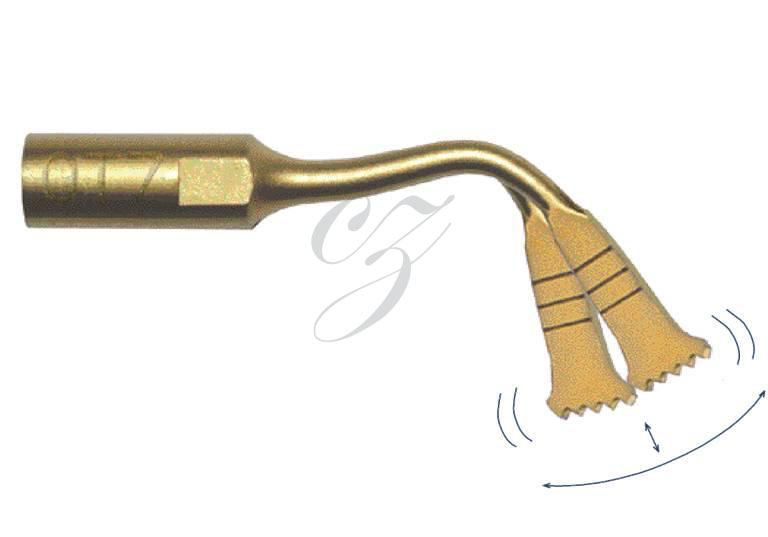
\includegraphics[width=0.3\columnwidth]{images/piezoChirurgie.png}
				\caption{		 
					Piezo-Chirurgie: Applikator erfährt durch Wechselspannung eine Längenänderung \cite{piezoChirurgie}.}
				\label{fig:piezoChirurgie}
			\end{figure}
	
	\section{Ausblick}
	 
		Die Hochfrequenzchirurgie genießt hohe Akzeptanz und Beliebtheit in den Operationssälen und entwickelt sich stetig weiter. Das Paper \cite{dual} stellt beispielsweise ein in Abbildung \ref{fig:dual} ersichtliches doppelseitiges Handstück vor, welches ein automatisches Wechseln mit einer simplen Handbewegung erlaubt. Das beidseitige Handstück soll eine einfache und sichere Alternative zu traditionellen Methoden darstellen, das ein hastiges Wechseln der Applikatoren erübrigt.
		\begin{figure}[ht] 
			\centering
			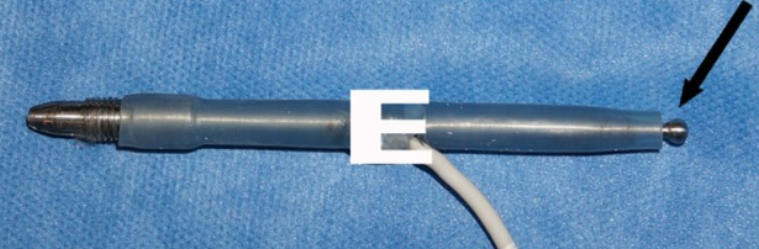
\includegraphics[width=0.35\columnwidth]{images/dual.png}
			\caption{Doppelseitiges Handstück: Linke Seite mit Applikatorfassung versehen, rechte Seite mit kugelförmiger Applikation zum Koagulieren bestückt \cite{dual}.}
			\label{fig:dual}
		\end{figure}\\
		Auch drahtlose Fußschalter (z.B. auf Bluetooth-Basis), wie sie die Firma \emph{Herga Technology} anbietet, dürften in Zukunft zur Eingabe der Steuerung eine immer größere Rolle spielen. Hierbei muss sich jedoch die Wirtschaftlichkeit der Geräte noch beweisen.
		
		Minggao Li und Xinggang Jiang stellen in ihrem Paper \cite{waterCool} ein wasserkühlendes System vor, bei denen spezielle Handgriffe (siehe Abbildung \ref{fig:waterCool}) zum Einsatz kommen. Dabei strömt das Kühlmittel von der Applikatorspitze zur chirurgischen Gewebeschnittstelle und reduziert Gewebewärme. Experimentelle Ergebnisse zeigen, dass das Wasserkühlungssystem den Gewebeschaden um mindestens $\SI{100}{\mu\meter}$ an Schichtdicke im Vergleich zur gewöhnlichen Aperatur bei gleicher Ausgangsleistung reduziert.
		\begin{figure}[h!] 
			\centering
			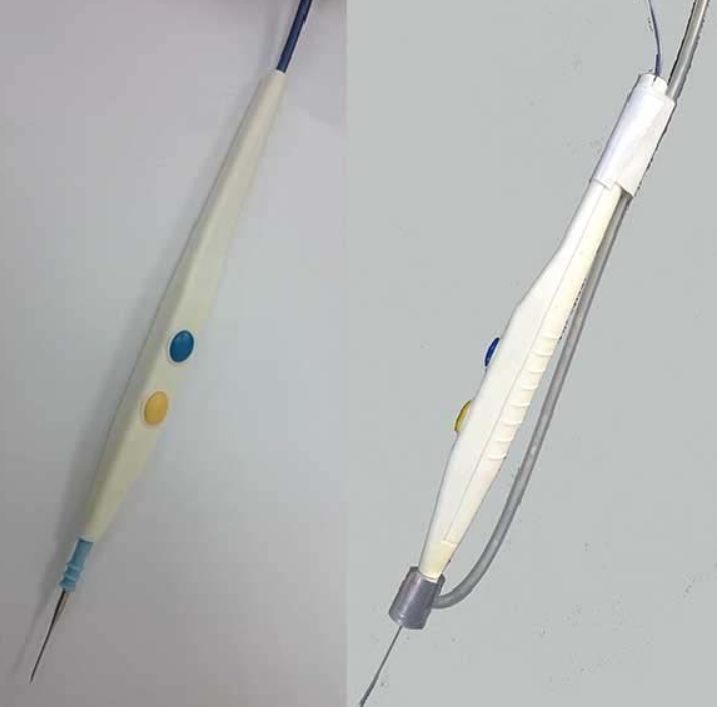
\includegraphics[width=0.3\columnwidth]{images/waterCool.png}
			\caption{Links: herkömmlicher Handgriff; Rechts: Handgriff besitzt ein Kühlschlauchsystem \cite{waterCool}.}
			\label{fig:waterCool}
		\end{figure}
		
		Auch wird die Integration von HF-Geräten in OP-Systeme über Kommunikationsnetzwerke einen Beitrag leisten, um über eine gemeinsame Bedienoberfläche alle für eine OP benötigten Geräte steuern zu können. Mögliche Ansteuerungselemente könnten hierbei ein Touchscreen oder die Sprachsteuerung sein \cite{kramme2016medizintechnik}.
		
		

	\newpage
	\bibliographystyle{unsrt}
	\bibliography{Literatur}
		
	\newpage	
	\section*{Zusammenfassung}
	
		Unter der Hochfrequenzchirurgie versteht man den assistierenden Einsatz von elektrischer Energie in der Chirurgie zur thermisch induzierten Veränderung oder Zerstörung von Gewebezellen mit dem Ziel der Hämostase (Blutstillung), Gewebedurchtrennung oder -versiegelung.
		
		Die HF-Chirurgie lässt sich grundsätzlich auf drei wichtige Bauteile, dem \emph{Hochfrequenzgenerator}, dem \emph{Handstück mit Applikator} und der \emph{Erdung} beschränken. Hierbei sorgt der HF-Generator für den benötigten Wechselstrom. Diese sind in der Lage eine Frequenz von $f>\SI{300}{\kilo\hertz}$ zu betreiben. Derart hohe Frequenzen sind nötig um faradische Effekte in den Muskeln und Nerven zu verhindern (Zucken, Herzrythmusstörung) und um die elektrische Energie effektiv auf das Gewebe zu übertragen. Applikatoren als Handwerkszeug und Stromspitze können je nach Anwendung in verschiedenen Bauformen auftreten. Hier kann ein isoliertes Handstück diverse Applikatorspitzen für den jeweiligen Einsatz aufnehmen. Die Erdung erfolgt mithilfe einer großflächigen Ableitelektrode oder einer Negativspitze (Pinzettenapplikator).\\
		
		Grundsätzlich kann das Gewebe verschiedene Formen, je nach thermischer Energieeinspeisung, annehmen. Hierbei sind die für die HF-Chirurgie zwei relevanten Formen die Denaturierung (Koagulation, Blutstillung, Gewebeversiegelung) und das Verdampfen (Schneiden, Abtragen) des Gewebes. 
		
		Beim Verdampfen/Schneiden wird ein sinusförmiger Wechselstrom generiert und kann je nach Schnittanforderung (sauberer Schnitt oder grober Schnitt mit Koagulation) modeliert werden. Hier kommen messerspitze Applikatoren zum Einsatz, welche eine hohe Stromdichte aufgrund der kleinen Kontaktfläche aufweisen. 
		
		Beim Denaturieren/Koagulieren wird das Gewebe lediglich ausgetrocknet und versiegelt, weshalb ein  großflächiger Applikator (z.B. Kugelaufsatz) zum Einsatz kommt um die Stromdichte zu senken. Der benötigte Strom wird durch eine Reihe diskontinuierlicher Wellenpakete erreicht, bei denen Ruhephasen die sinusförmigen Wellenzyklen unterbrechen und die Gewebebildung ein wenig abkühlen lassen.\\
		
		Die verschiedenartigen Anwendungsformen können prinzipiell in \emph{bipolare und monopolare Verfahren} eingeteilt werden. Für die Erzeugung eines elektrischen Stroms benötigt man grundsätzlich zwei Elektroden mit je einem +Pol und -Pol. 
		
		Bei der bipolaren Technik besitzt der Applikator zwei Spitzen, ähnlich einer Pinzette, zwischen denen die Spannung anliegt. Das zu bearbeitende Gewebe wird zwischen den Pinzettenspitzen genommen und stellt so einen Stromfluss durch das Gewebe her. 
		
		Bei der monopolaren Technik fließt der Strom zwischen Applikatorelektrode und einer großflächigen Ableitgegenelektrode (angebracht an Oberschenkel oder Rücken des Patienten), wobei die Stromdichte an der Applikatorelektrode sehr hoch ist, sodass thermische Effekte auftreten.
		Die Stromdichte nimmt hin zur Aktiven Elektrode quadratisch zu, das bedeutet außerhalb des Wechselwirkungvolumens fächern sich die E-Feldlinien derart auf, dass die Stromdichte für nicht relevante Körperstellen unkritisch ist.
			
		
\end{document}